\section{Development of the formal kernel: initial conditions, geometry, and refinement}
\label{sec:extension}

The eighty-one-position support does not coincide with the domain of initial conditions for the dynamics. An initial condition must also specify an orientation, and the additive and multiplicative sheets have independent cursors. This distinction allows exhaustive reconstruction of the emission without selecting a numerical region in advance.

\subsection{Initial states and the emission recurrence}

For enumeration we use indices \(I_9=\{0,\ldots,8\}\), related to positive labels by \(i\mapsto i+1\). Let
\[
 \mathcal S=I_9^2\times\{N,E,S,O\},\qquad
 \Omega_{\rm seed}=\mathcal S_+\times\mathcal S_\times.
\]
Each initial condition \(\omega=(s_+,s_\times)\) determines two positions and two directions. The domain comprises all ordered pairs, so
\begin{equation}
 |\mathcal S|=324,\qquad |\Omega_{\rm seed}|=324^2=104\,976.
 \label{eq:semillas}
\end{equation}
The independent annex enumerates all these conditions; the body presents the law transforming them. The rows of an emission table are fibers of this initial-condition domain.

The finite realization uses six windows of nine transitions. At each instant \(t\), the phase signature is \(M_{\rm ph}(1+((t-1)\bmod9))\). If its value is \(+1\), the positive residue \(\Sigma(i+1,j+1)=\rho_9(i+j+2)\) of the first cursor is read and that cursor is then moved; if its value is \(-1\), the positive residue \(\Pi(i+1,j+1)=\rho_9((i+1)(j+1))\) of the second cursor is read and the second cursor is then moved. Zero increments the neutral counter. At the end of transitions twenty-seven and fifty-four, cardinal orientations are reversed. Integer evaluations and their quotients are retained in the record, but the emitter uses the residue readings specified here.

In the unit sector, the multiplicative reader uses the base-two discrete logarithm in \((\ZZ/9\ZZ)^\times\):
\[
 \ell_9(1)=0,\quad\ell_9(2)=1,\quad\ell_9(4)=2,\quad
 \ell_9(8)=3,\quad\ell_9(7)=4,\quad\ell_9(5)=5.
\]
For finite emission it is extended by zero to the non-unit sector. This extension is an observable, not an identification of the elements \(3,6,9\) with the multiplicative identity. The sheet and its membership in the radical sector remain in the trajectory record.

Let \(S_m\) be the sum of the three positive additive residues \(\Sigma\) in window \(m\), \(E_m\) the sum of the three discrete exponents of the multiplicative residues \(\Pi\), and \(Z_m=3\) the number of neutral events. Thus \(S_m\) does not sum the integer evaluations \(S=i+j\), whose quotients remain in the record. With \([a]_{10}\in\{0,\ldots,9\}\), the decimal emission rule is
\begin{align}
 d_{m,1}&=[S_m]_{10},\notag\\
 d_{m,2}&=[S_m+E_m]_{10},\notag\\
 d_{m,3}&=[3S_m+5E_m+7Z_m]_{10},\notag\\
 U_m&=100d_{m,1}+10d_{m,2}+d_{m,3}.
 \label{eq:emisor-seis}
\end{align}
The integer coefficients and calendar of this recurrence are explicit parts of the declared emission law. Values of \(\pi,\varphi,e\) or \(\alpha\) are not received. Distinguishing an emission rule from a constant recognized from its output prevents the genealogy from being hidden in a decimal table.

If \(s_m=[S_m]_{10}\) and \(e_m=[E_m]_{10}\), the same rule is written
\begin{equation}
 U_m=100s_m+10[s_m+e_m]_{10}+[3s_m+5e_m+1]_{10}.
 \label{eq:acoplamiento}
\end{equation}
The final one is the residue of \(7Z_m=21\) modulo ten. The oriented ternary reduction of the catalog adopts the convention
\begin{equation}
 \Psi(U_1,\ldots,U_6)=([-U_1]_3,\ldots,[-U_6]_3).
 \label{eq:psi-catalogo}
\end{equation}
The sign of this chart is explicit: changing it modifies the words and requires transport of subsequent orientations. The balanced identification of each component of \(\FF_3\) with TRIT is performed after \eqref{eq:psi-catalogo}.

\begin{proposition}[Injective factorization of emission]
The word \(U=(U_1,\ldots,U_6)\) determines both signatures \(s=(s_1,\ldots,s_6)\) and \(e=(e_1,\ldots,e_6)\). The emission image has \(18\cdot26=468\) elements. The ternary projection has \(243\) distinct values in the ambient set of \(729\) words.
\end{proposition}
\begin{proof}
The hundreds digit of \(U_m\) recovers \(s_m\). If \(b_m\) is its tens digit, then \(e_m=[b_m-s_m]_{10}\). The units digit checks the third congruence of \eqref{eq:acoplamiento}. Hence coupling is injective on the signature product.

Enumerating the \(324\) conditions for one cursor through the preceding recurrence produces eighteen additive signatures, each with eighteen preimages, and twenty-six multiplicative signatures, of which twenty-four have eight preimages, one has twenty-four, and one has one hundred and eight. The annex preserves these signatures and their initial conditions, allowing the finite enumeration to be repeated without a reference numerical catalog. Injectivity of the coupling gives \(18\cdot26\) emissions and multiplicities
\[
 \underbrace{432}_{18\cdot24}\text{ fibers of }144,
 \qquad18\text{ fibers of }432,
 \qquad18\text{ fibers of }1944.
\]
The sum is \(432\cdot144+18\cdot432+18\cdot1944=104\,976\). Applying \eqref{eq:psi-catalogo} to the \(468\) emissions produces exactly \(243\) words. This last number is the cardinality of the image, not of the space \(\FF_3^6\).
\end{proof}

This factorization explains the difference between finite exhaustiveness and unlimited depth. Domain \eqref{eq:semillas} is complete for the declared support and emitter; it does not contain every prefix of every prolongation in advance. Depth belongs to the system of compatible extensions constructed over those conditions.

\subsection{Calendar closure and memory advance}

The calendar of one hundred and eight transitions consists of twelve nonadic windows. Its group structure is more precise than an informal product of two periods:
\begin{equation}
 0\longrightarrow C_{12}\xrightarrow{\iota}C_{108}
 \xrightarrow{p}C_9\longrightarrow0,
 \quad\iota([b])=[9b],\quad p([t])=[t]_9.
 \label{eq:extension108}
\end{equation}
If \(t=9b+r\) with \(0\le r<9\), adding two phases produces the carry
\[
 (b,r)+(b',r')=
 \left(b+b'+\left\lfloor\frac{r+r'}9\right\rfloor,\ [r+r']_9\right),
\]
where the first coordinate is reduced modulo twelve. Composition preserves the term linking the two coordinates.

\begin{proposition}[Nonsplitting of the calendar]
Sequence \eqref{eq:extension108} is exact and admits no section that is a group homomorphism.
\end{proposition}
\begin{proof}
The kernel of reduction modulo nine is the subgroup of multiples of nine, the image of \(\iota\). If the extension split, commutativity would give \(C_{108}\cong C_{12}\times C_9\). The first group has exponent \(108\), whereas the second has exponent \(\operatorname{lcm}(12,9)=36\), a contradiction.
\end{proof}

Nine transitions restore the nonadic phase and advance one window; one hundred and eight restore the finite calendar. Neither fact requires erasing the trajectory or restoring a prolongation prefix. Nonadic holonomy \(\Gamma_9\) denotes transport through one turn on states with memory, so that
\begin{equation}
 g(\Gamma_9x)=g(x),\qquad M(\Gamma_9x)=M(x)+1.
 \label{eq:holonomia-memoria}
\end{equation}
Phase equality and memory increment are compatible and constitute two observations of the same transport.

% Recovery of 02_trit_geometrias and holonomy with memory.
\subsubsection{Temporal parametrization of compatibility and tritic orientation}
\label{trit-temporal-compatibilidad}

The temporal interpretation of TRIT is established on transitions of the
complete state. Let \(x\xrightarrow{\rm adm}y\) be the admissibility relation
determined by TPK operations on \(\widehat X\). A trajectory parametrized
by a discretely ordered set \(\mathcal T\) is a map
\[
 \gamma:\mathcal T\longrightarrow\widehat X,\qquad
 \gamma(t)\xrightarrow{\rm adm}\gamma(t^+),
\]
where \(t^+\) is the successor of \(t\). The compatibility relation
precedes the choice of parameter: the order allows its transitions to
be expressed as an evolution. When the term section is used, the
projection \(p:E\to\mathcal T\) and condition
\(p\circ\gamma=\operatorname{id}_{\mathcal T}\) are also declared.
The state space, temporal order, and transported information are thereby specified.

The signature \(\tau\) selects a quadratic regime and admits a temporal
reading relative to this parametrization. Type \(+1\), with
\(J_{+1}^{2}=-I\), represents return and memory; type \(0\), with
\(J_0^{2}=0\), represents the transition threshold; type \(-1\), with
\(J_{-1}^{2}=I\), represents opening in two eigendirections. In the
model's temporal terminology, these functions correspond, respectively,
to past, present, and future. The correspondence concerns the operational
position of a transition within a history: retained antecedent, update,
and admissible prolongation.

This interpretation acquires content through three distinct operations.
Restriction of a trajectory recovers the prefix already constructed.
The update \(\mathcal U_t\) composes selection, transport, and recording
in the observed transition. Prolongation considers continuations that
preserve the boundary conditions of that prefix. If
\(\mathcal P_n(x)\) denotes the set of admissible continuations of
length \(n\) from \(x\), deleting the last step defines
\[
 r_n:\mathcal P_{n+1}(x)\longrightarrow\mathcal P_n(x).
\]
An unlimited continuation is a collection \((\gamma_n)_{n\geq1}\)
satisfying \(r_n(\gamma_{n+1})=\gamma_n\). The inverse system thus
preserves the restrictions each depth imposes on preceding depths.
Existence of a compatible collection is established in the corresponding
prolongation domain; merely specifying the sets \(\mathcal P_n(x)\)
does not replace that proof.

Bidirectionality therefore combines reconstruction of antecedents with
compatibility of continuations. On the signature sequence, the involution
\(C_{\rm rev}\) reverses order and changes the sign of each component.
The trajectory is also subject to the transformations of position, sheet,
and boundary specified by transport. The reversed signature is an
observation of the conjugate trajectory, not a replacement for its other
coordinates. The threshold remains distinguished: the visible value
\(0\) retains its transition function even when its quotient or
historical record is nonzero.

The relation with exponential geometries is equally precise. In each
fixed regime, \(\exp(tJ_\tau)\) composes parameters and preserves the
algebraic norm. Elliptic closure belongs to that local representation.
Phase return of \(\Gamma_9\), by contrast, acts on the trajectory
with memory, according to \eqref{eq:holonomia-memoria}. A trajectory
can recover its phase while retaining a new antecedent: historical data
have changed although the phase observation is the same. The parabolic
threshold retains a linear displacement; hyperbolic opening separates
two eigendirections of expansion and contraction. These three
realizations provide composition laws, whereas the TPK determines their
selection and effective concatenation.

The aperiodic suspension in Section \ref{sec:generacion} will make this
distinction explicit through a finite phase factor, an irrational rotation,
and a memory degree. The link between TRIT and temporality is thus
expressed by operations on trajectories and their quadratic representations.
Its content exceeds a classification of signs: it preserves the regime,
the direction of transport, and the relation between antecedent,
transition, and continuation.


The monodromic representation of this return is developed in
Section~\ref{mono-ampl:conexion}. There, the holonomy of the state
is distinguished from its representation on phase and counter. The
symbolic suspension in Section~\ref{mono-ampl:cristal} defines the
aperiodic time-crystal model, and Section~\ref{mono-ampl:euler}
composes this temporality with the three Euler realizations.

\subsection{Observable compression and orthogonal conservation}

An isometric realization provides a quantitative expression of what a reduced observation loses. Let \(U:\mathcal H\to\mathcal H\) be an isometric realization of transport through one turn, \(U^*U=I\), and \(J:\mathcal H_{\rm vis}\to\mathcal H\) an isometric inclusion. Define
\[
 T=J^*UJ,\qquad D=(I-JJ^*)UJ.
\]
Then
\begin{equation}
 UJ=JT+D,\qquad J^*D=0,\qquad I-T^*T=D^*D.
 \label{eq:conservacion-ortogonal}
\end{equation}
The last equality follows by taking the adjoint product of the first and using orthogonality. Contraction of the visible component does not by itself constitute destruction of information in the total state.

\begin{proposition}[Finite-horizon conservation]
If \(I-T^*T=D^*D\), then, for every \(n\ge1\),
\begin{equation}
 I=\sum_{r=0}^{n-1}T^{*r}D^*DT^r+T^{*n}T^n.
 \label{eq:telescopia}
\end{equation}
\end{proposition}
\begin{proof}
Multiplying \(D^*D=I-T^*T\) by \(T^{*r}\) and \(T^r\), then summing, produces a telescoping sum. The interior terms cancel, leaving \(I-T^{*n}T^n\).
\end{proof}

The final summand preserves the terminal state. Removing it before justifying a limit would alter the equality. This distinction is the operational content of conservation of unity under compression: the norm is distributed among the visible component, memory, and terminal, rather than being replaced by a single residue.

\subsection{Local development: commutation, Lorentzian signature, and discrete curvature}
\label{vii:sec:bloque-compresion}

The adjacent diagonal block with equal diagonals modulo nine is unique. Indeed,
\[
 k^2\equiv(k+1)^2\pmod9\quad\Longleftrightarrow\quad2k+1\equiv0\pmod9
\]
gives \(k=4\). Its visible matrix is
\[
 B_c=\begin{pmatrix}7&2\\2&7\end{pmatrix}=7I+2R,
 \quad R=\begin{pmatrix}0&1\\1&0\end{pmatrix},\quad R^2=I.
\]
With \(P_\pm=(I\pm R)/2\), one obtains \(B_c=9P_++5P_-\). The unity of stochastic normalization and conservation of an indefinite form are two realizations of this block:
\[
 \frac{B_c}{9}=P_++\frac59P_-,\qquad
 \frac{B_c}{\sqrt{45}}=\exp(\eta R),\quad\eta=\frac12\log\frac95.
\]
For \(Q=\operatorname{diag}(1,-1)\), the second matrix satisfies \(B_c^{\mathsf T}QB_c=45Q\). This yields a local realization in \(SO^+(1,1)\); no prior introduction of four-dimensional spacetime is required to prove it.

Uniform averaging over the classes \(C_1=\{1,4,7\}\), \(C_2=\{2,5,8\}\), and \(C_0=\{3,6,9\}\) gives
\[
 M_\Pi=\begin{pmatrix}4&5&6\\5&4&6\\6&6&9\end{pmatrix},\quad
 M_\Sigma=\begin{pmatrix}5&6&4\\6&4&5\\4&5&6\end{pmatrix}.
\]
The characteristic polynomial of \(M_\Pi\) is
\[
 (\lambda+1)((\lambda-9)^2-72),
\]
so its quadratic form has signature \((2,1)\). The local spectral gap \(9-5=4\), the coefficient \(2\), the aggregate difference \(51-45=6\), and the integrated defect \(9\cdot6=54\) describe different levels of the same arithmetic comparison. They are not interchangeable indices of a single operator.

Discrete curvature can be described directly before this spectral realization. In residues, let \(S(x,y)=x+y\), \(P(x,y)=xy\), and let \(\Delta_x,\Delta_y\) be forward differences. Link variables are differences of potentials, \(A_x^T=\Delta_xT\), \(A_y^T=\Delta_yT\), and we set
\[
 F(T_x,T_y)=\Delta_x\Delta_yT_y-\Delta_y\Delta_xT_x.
\]
Since \(\Delta_xS=\Delta_yS=1\), \(\Delta_xP=y\), and \(\Delta_yP=x\),
\begin{equation}
 F(S,S)=F(P,P)=0,\qquad F(S,P)=+1,\quad F(P,S)=-1\pmod9.
\end{equation}
Sum and product, taken separately, induce flat connections; their ordered mixture changes the sign of plaquette curvature. Summing over a rectangle of sides \(a,b\) cancels interior edges, and the oriented boundary sum equals \(\pm ab\) modulo nine. An exact relation thus appears between composition order and boundary orientation.

\subsection{Cubic completion and two notions of boundary}

Expanding the cubic support of side nine to that of side ten admits an exact positional stratification:
\begin{equation}
 10^3=9^3+3\cdot9^2+3\cdot9+1=729+243+27+1.
 \label{eq:cubo}
\end{equation}
The first term corresponds to three interior coordinates; the second to one new coordinate; the third to two; and the last to the vertex with three new coordinates. The expansion corona contains \(271\) positions. By contrast, the internal boundary of the discrete cube of side nine contains \(9^3-7^3=386\). The difference between these counts is a difference of domain, not a conflict of values.

Dividing \eqref{eq:cubo} by \(1000\) gives a normalized partition of unity. Cube incidence distinguishes six faces, twelve edges, and eight vertices. The connection to Steiner hexads and octads is realized through the combinatorial maps of Section~\ref{exc:seccion}, which preserve the cardinalities and incidence of each domain. This completion fixes the relation between bases \(729\) and \(1000\) here; the numerical generation in Section~\ref{sec:generacion}, the electronic coordinate \(\rho_E=\varphi/\pi^2\) in \eqref{eq:areal-electron}, and the exceptional prolongation subsequently form three typed outputs, while the gravitational construction reuses the action sections derived from that genealogy in Section~\ref{v:ant:sec:action}.

\subsubsection{Stratification of the completion and restoration of the apex}
\label{sec:revision-emrh}

The completion admits a set-theoretic description making its operation
explicit. Let \(E_9\) be the set of nine residue classes, represented
positively by \(1,\ldots,9\), and let \(\ast\) be an additional element.
The symbol \(\ast\) differs from the zero class, already represented by \(9\).
Consequently, extending \(E_9\) to
\(\widehat E=E_9\sqcup\{\ast\}\) increases the cardinality from nine
to ten without changing the internal modular identification. The cubic
completion is \(\widehat C=\widehat E^3\), and the initial cube is \(C=E_9^3\).

\begin{definition}[Strata of combinatorial codimension]
For \(0\leq r\leq3\), define
\[
 S_r=\{(x_1,x_2,x_3)\in\widehat E^3:
             \#\{j:x_j=\ast\}=r\}.
\]
The apex of the completion is \(a_\ast=(\ast,\ast,\ast)\), and the
punctured completion is \(\widehat C^{\circ}=\widehat C\setminus\{a_\ast\}\).
\end{definition}

\Needspace{10\baselineskip}
\begin{proposition}[Exact decomposition of the completion]
The strata are disjoint and satisfy
\begin{align}
 \widehat C&=S_0\sqcup S_1\sqcup S_2\sqcup S_3,
 &|S_r|&=\binom3r9^{3-r},\label{eq:revision-estratos}\\
 |\widehat C^{\circ}|&=729+243+27=999,
 &|\widehat C|&=999+1=1000.\label{eq:revision-999}
\end{align}
The punctured expansion contains \(270\) elements in addition to the
initial cube; the complete expansion contains \(271\).
\end{proposition}
\begin{proof}
An element of \(S_r\) is obtained by choosing the \(r\) coordinates
containing \(\ast\), in \(\binom3r\) ways, and assigning one of the
nine classes of \(E_9\) to each remaining coordinate. Classification by
the number of additional coordinates is exhaustive and its classes are
disjoint. The sole element of \(S_3\) is \(a_\ast\). Removing it
subtracts one from the total cardinality; restoring it recovers the
complete Cartesian product.
\end{proof}

The expression \emph{holographic extreme and mean ratio}, abbreviated EMRH
in the corpus, here denotes this articulation of the initial body, expansion
strata, and unit restoration. Its immediate content is the exact partition
of a finite product and its normalization. The number \(999\) represents
a definite object, the punctured completion; \(1000\) represents its
closure through restoration of the apex. The added unit therefore has
an explicit incidence location.

\begin{figure}[htbp]
\centering
\begin{tikzpicture}[x=1cm,y=1cm,>=Stealth,font=\small]
\draw[->] (0,0)--(12.4,0);
\foreach \x/\a/\b in {0/729/{S_0},4.0/243/{S_1},7.5/27/{S_2},10.6/1/{S_3}}{
  \draw (\x,0.12)--(\x,-0.12);
  \node[above=5pt] at (\x,0) {\(\a\)};
  \node[below=5pt] at (\x,0) {\(\b\)};
}
\draw[decorate,decoration={brace,amplitude=5pt}] (0,1)--(7.7,1);
\node[above=8pt] at (3.85,1) {Punctured completion: \(999\)};
\draw[decorate,decoration={brace,mirror,amplitude=5pt}] (0,-1)--(10.8,-1);
\node[below=8pt] at (5.4,-1) {Full completion: \(1000=999+1\)};
\node[align=center] at (10.6,1.5) {Apex\\\((\ast,\ast,\ast)\)};
\end{tikzpicture}
\caption{Strata of the cubic completion. The arrangement represents
the set-theoretic decomposition, not a metric scale. The \(243\) elements
of \(S_1\) form three coordinate strata of \(81\) elements; the \(27\)
elements of \(S_2\) form three strata of \(9\). The apex completes the partition.}
\label{fig:revision-emrh}
\end{figure}

% Geometric adaptation of the preserved cubic-completion figure.
\begin{figure}[htbp]
\centering
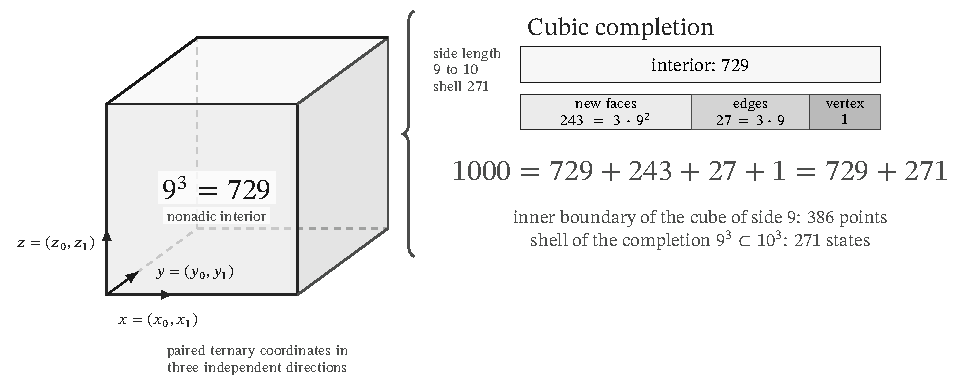
\includegraphics[width=\textwidth]{figures/cubo_emrh.pdf}
\caption{Cubic representation of the expansion from nine to ten classes per coordinate. Strata \(S_1,S_2,S_3\) locate the added incidences on faces, edges, and the apex; their cardinalities form the \(271\)-element shell. The \(386\)-element boundary belongs to the initial cube. This geometric perspective complements the partition in Figure~\ref{fig:revision-emrh}; graphical spacing is schematic.}
\label{fig:completacion-cubo-recuperado}
\end{figure}


\subsubsection{Conservation of unity and dimensional compatibility}

Normalization is not limited to dividing an isolated identity. In dimension
\(d\), the product \(\widehat E^d\) carries the uniform measure
\(\mu_d(\{x\})=10^{-d}\). The coordinate projection
\(p_d:\widehat E^{d+1}\to\widehat E^d\) deletes the last coordinate.

\begin{proposition}[Projective compatibility of normalized measures]
For every \(d\geq1\),
\[
 (p_d)_*\mu_{d+1}=\mu_d,
 \qquad \mu_d(\widehat E^d)=1.
\]
The mass of the stratum with \(r\) additional coordinates is
\(\binom dr9^{d-r}/10^d\), and the masses of all strata sum to one.
\end{proposition}
\begin{proof}
Each point of \(\widehat E^d\) has ten preimages. Their total mass is
\(10\,10^{-(d+1)}=10^{-d}\). Equality for any subset follows by
summing over its points. The stratified formula follows from the same
count as \eqref{eq:revision-estratos}; the binomial
\((9+1)^d\) gives total normalization.
\end{proof}

In dimension three, removing the apex leaves mass \(999/1000\), and
restoring it adds \(1/1000\). Renormalizing before restoration would
define a different measure: the distinction is operationally relevant.
In particular, conservation of probability mass, conservation of transport
records, and thermodynamic dissipation concern different objects. The
proposition proves the first and provides the compatible support for
studying the second; the third requires a specified dynamic and energetic realization.

The internal geometric boundary also remains distinct.
On the Cartesian representative \(\{1,\ldots,9\}^3\), removing
\(\{2,\ldots,8\}^3\) leaves \(386\) points. This boundary belongs
to the initial cube, whereas \(\widehat C\setminus C\) belongs to
its expansion. Cubic completion, base-thousand positional expansion,
and exceptional-incidence reading share support data; their respective
maps determine which information from these data each representation uses.


\subsection{Cubic incidence and Lorentzian realization}

Cubic completion supplies a relation between interior and boundary.
Its geometry can be developed through incidence of the six faces with
the eight vertices. Label faces by \((i,\varepsilon)\),
\(i\in\{1,2,3\}\), \(\varepsilon\in\{+1,-1\}\), and vertices by
\(\nu\in\{+1,-1\}^3\). The incidence matrix is
\[
 M_{(i,\varepsilon),\nu}=\mathbf1_{\{\nu_i=\varepsilon\}}.
\]
Let \(u=(1,\ldots,1)^{\mathsf T}\in\RR^6\), let \(R_F\) denote
face opposition, and let \(P_u=uu^{\mathsf T}/6\), \(P_-=(I-R_F)/2\).

\begin{proposition}[Four-dimensional incidence quotient]
The incidence Gram matrix satisfies
\[
 MM^{\mathsf T}=12P_u+4P_-.
\]
Its eigenvalues \(12,4,0\) have multiplicities \(1,3,2\).
Consequently,
\[
 Q_\square=\RR^6/\ker(MM^{\mathsf T})
 \simeq\RR u\oplus E_-,\qquad E_-=\operatorname{im}P_-.
\]
\end{proposition}
\begin{proof}
A face contains four vertices; two opposite faces have empty intersection,
and two distinct non-opposite faces share two vertices.
The matrix \(12P_u+4P_-\) has exactly these entries.
The uniform subspace has dimension one; differences between opposite
faces generate a three-dimensional space orthogonal to it.
Its complement has dimension two and belongs to the kernel.
\end{proof}

The decomposition \(1+3\) comes from incidence. The temporal choice
is declared through the bilinear form
\[
 B_\square([x],[y])=\langle x,(P_--P_u)y\rangle.
\]
It is well defined on the quotient because both projectors annihilate
the kernel. In the basis
\[
 t=[u]/\sqrt6,\qquad
 d_i=[e_{i,+}-e_{i,-}]/\sqrt2,
\]
its matrix is \(\operatorname{diag}(-1,1,1,1)\). The domain,
decomposition, and sign convention producing the Minkowski realization
are thus explicit. The positive Gram matrix determines the quotient;
the temporal assignment determines the indefinite form on it.

The operator
\[
 W_\square=\sqrt6P_u+\sqrt2P_-,\qquad
 W_\square e_{i,\varepsilon}=t+\varepsilon d_i
\]
sends the six face labels to null directions, since
\(B_\square(t+\varepsilon d_i,t+\varepsilon d_i)=-1+1=0\).
Direction reversal and face opposition thus acquire a concrete
geometric realization.

\subsubsection{Soldering, reversal, and subdivision}

The cellular realization uses an invertible transport \(U_m(a)\),
preserving the Lorentzian form, between the endpoint fibers of an
oriented dual edge \(a\), a face label \(\lambda_m(a)\),
and an orientation \(\sigma_m(a)\).
With \(\ell_m=\ell_0/9^m\), the soldering map is
\[
 \beta_m(a)=\ell_m\sigma_m(a)
 W_{\square,s(a)}e_{\lambda_m(a)}.
\]
Compatible reversal satisfies
\[
 \beta_m(\bar a)=-U_m(a)\beta_m(a).
\]
Identify the source fibers at two consecutive levels through the declared
refinement isometry. If the nine subsegments \(a_1,\ldots,a_9\),
at level \(m+1\), preserve label and orientation when transported
to that common fiber, then
\begin{equation}
 \beta_m(a)=\sum_{j=1}^9
 U_{m+1}(a_1\cdots a_{j-1})^{-1}\beta_{m+1}(a_j).
 \label{eq:soldadura-refinamiento}
\end{equation}
Each transported term equals \(\ell_m/9\) times the same null
direction, proving the identity. The compatibility hypothesis determines
which subdivisions realize this refinement. The equation brings together
direction, scale, and transport, rather than limiting geometric
correspondence to a dimension count.

With orientation and the Lorentzian form also fixed, Hodge duality
on \(\Lambda^2Q_\square^*\) satisfies \(\star^2=-I\).
In dimension four, the sign is \((-1)^{2(4-2)+1}=-1\).
This yields a real complex structure on two-forms and, after
complexification, the eigenspaces with eigenvalues \(+i\) and \(-i\).
The electronic application in Article I constructs its persistent section
on the pair of APP sheets and fixes the polarity entering the
electromagnetic realization. In this article, the declared orientation and
Lorentzian form transport that structure to the gravitational domain:
Hodge duality organizes the components of the current, and
Section~\ref{vii:sec:corriente-respuesta-cartan} incorporates them into the
algebraic Cartan--Holst equation.

\subsection{Compatibility of modular and positional reductions}

The block-decimal base enters through Euclidean division preserving
residue and quotient simultaneously:
\[
 n=1000q+r,\qquad 0\le r<1000.
\]
Since \(1000\equiv1\pmod9\) and \(1000\equiv1\pmod3\),
\[
 n\equiv q+r\pmod9,\qquad n\equiv q+r\pmod3.
\]
Reduction of a block therefore requires the quotient's contribution
to recover the integer's class. The numbers \(0\) and \(1000\)
have the same remainder modulo \(1000\), but different classes
modulo \(9\) and \(3\). This is an operational reason for preserving
memory through a change of resolution.

Ternary refinement and determination of a decimal prefix can be
coordinated through a single integer remainder. If \(N/3^L\)
is a cylinder endpoint and \(D/1000^r\) a decimal endpoint, define
\[
 A=1000^rN-D3^L.
\]
On adding six ternary symbols, \(N'=729N+\nu\),
\(L'=L+6\), with \(0\le\nu<729\). If the decimal prefix remains
fixed, one obtains
\[
 A'=729A+\nu1000^r.
\]
If a decimal block \(\delta\) is also incorporated, then
\(D'=1000D+\delta\), \(r'=r+1\), and
\begin{equation}
 A'=729000A+\nu1000^{r+1}-729\delta3^L.
 \label{eq:residuo-dos-bases}
\end{equation}
Both identities follow by substitution of the definitions. Comparing
endpoints is thus reduced to integer operations retaining each
prolongation's contribution. This compatibility makes it possible
to refine a region before evaluating its real coordinate.

% Incorporation at the end of extension.tex; contains no main section.
% Provenance: RESULTADO_RECUPERADO; sector-specific explicit statement of hypotheses.
% Sources read: Doble proyección holográfica monograph (editorial source material),
% manuscrito/local/01_tesis_recuperada.tex and
% manuscrito/generated/algebra_holonomica.tex, especially §§1--7 and 21.
% Governing definition of number: manuscrito/flattened/main_autosuficiente.tex,
% sections starting at lines 22137 and 23000 of the 775-page source collection.
% Its global presentation is not adopted as proof of every TPK arrow.

\subsection{Number as a compatible section and value as a reading}
\label{hist:seccion}

Distinguishing state from observation specifies what object is prolonged
as resolution increases. At depth \(n\), let \(X_n\) be the set of
admissible states produced by APP--TRIT--TPK. Their data include position,
sum and product sheets, residues and quotients, regime, orientation,
carry, phase, route, boundary, memory, and survival. These are not
independent coordinates: earlier arithmetic evaluations and transports
impose their relations. A prolongation preserves these relations in
each antecedent, even while adding new steps and memory data.
This is the meaning of the arithmetic of histories: the tritic selection and
cardinal transport of Section~\ref{tpk-int:seleccion}, the memory composition
of Section~\ref{tpk-int:memoria}, and the nonadic holonomy of
Section~\ref{tpk-int:holonomia} act on a single prolonged state.

Let \(r_{m,n}:X_m\to X_n\), for \(m\geq n\), be depth
restrictions, with \(r_{n,n}=\operatorname{id}\) and
\(r_{\ell,n}=r_{m,n}\circ r_{\ell,m}\). Each restriction preserves
the prefix and the information already determined in it.

\begin{definition}[Compatible numerical section]
An HMT number is a compatible history of the state system:
\begin{equation}
 x=(x_n)_{n\geq0}\in X_\infty:=\varprojlim_n X_n,
 \qquad r_{m,n}(x_m)=x_n.
 \label{hist:limite-inverso}
\end{equation}
A reader is an additional operation on a specified domain of these
histories. A digit is a finite observation; a scalar value is an evaluation
of the reader. The pair consisting of a section and its reader constitutes
a read presentation, not a redefinition of the section's identity.
\end{definition}

On the Archimedean domain \(X_\infty^{\mathrm{Arch}}\), the reader
associates a closed cylinder with each prefix, preserves nesting, and
makes its diameter tend to zero. It thus determines
\begin{equation}
 \operatorname{ev}_{\mathbb R}:X_\infty^{\mathrm{Arch}}\longrightarrow
 \mathbb R,\qquad
 \{\operatorname{ev}_{\mathbb R}(x)\}=\bigcap_n I_n(x).
 \label{hist:evaluacion}
\end{equation}
The concrete construction of these cylinders and the determination of
their boundaries are developed in Section~\ref{sec:generacion}.
Definition \eqref{hist:limite-inverso} does not by itself assert
that the image of \eqref{hist:evaluacion} is the entire line:
a coverage claim requires its own theorem. Nor does equality of
values establish equality of histories without an injectivity result.
This separation allows precision to be discussed as depth while preserving
the distinction between the arithmetic antecedent and its scalar realization.

\subsection{Composition of histories and memory multiplier}
\label{hist:algebra}

Fix a sector of states at depth \(n\) and a category \(\mathcal C\)
whose arrows are its admissible histories. Composition is written
\(vu=v\circ u\): first traverse \(u\), then \(v\).
Elementary steps come from TPK selection, transport, and updating.
A local tritic fiber admits the notation
\(\mathbb R[J_x]/(J_x^2+\tau(x)1_x)\), where
\(\tau(x)\in\{+1,0,-1\}\). Regime and orientation belong to
the transported state; a transition between regimes does not amount
to identifying their quadratic algebras.

The following formulation specifies an algebraic sector of this composition.
For each object \(x\), a unital associative real algebra \(A_x\),
possibly noncommutative, is given. For each \(u:x\to y\), a
unital homomorphism \(\rho_u:A_x\to A_y\) is given. Assume a strict action:
\begin{equation}
 \rho_{\operatorname{id}_x}=\operatorname{id}_{A_x},\qquad
 \rho_v\rho_u=\rho_{vu}.
 \label{hist:accion-estricta}
\end{equation}
For each composable pair \(u:x\to y\), \(v:y\to z\), fix an
invertible central multiplier \(\Omega(v,u)\in Z(A_z)^\times\).
Require the normalization
\(\Omega(\operatorname{id}_y,u)=\Omega(u,\operatorname{id}_x)=1_y\)
and, for every composable triple, the identity
\begin{equation}
 \rho_w\bigl(\Omega(v,u)\bigr)\Omega(w,vu)
   =\Omega(w,v)\Omega(wv,u).
 \label{hist:cociclo}
\end{equation}
These are explicit hypotheses on transports and their coefficients,
not a consequence of calling the dynamics holonomic. Applying this
presentation to a TPK sector requires identifying its \(\rho_u\)
and \(\Omega(v,u)\). Transitions expressed through bimodules require
preserving that structure and are not replaced by \eqref{hist:accion-estricta}.

The space of finite sums
\[
 \mathcal H(\mathcal C,A,\rho,\Omega)
   =\bigoplus_{u\in\operatorname{Mor}(\mathcal C)} A_{t(u)}T_u
\]
receives the bilinear product
\begin{equation}
 (aT_v)(bT_u)=a\rho_v(b)\Omega(v,u)T_{vu},
 \label{hist:producto}
\end{equation}
when the arrows are composable, and zero otherwise. Here \(t(u)\)
denotes the terminal state. Addition gathers histories with coefficients;
multiplication concatenates histories while preserving the record multiplier.

\begin{proposition}[Sectorial associativity with a central multiplier]
Under \eqref{hist:accion-estricta} and \eqref{hist:cociclo}, product
\eqref{hist:producto} is associative. If the object set is finite,
its identity is \(\sum_x1_xT_{\operatorname{id}_x}\).
\end{proposition}
\begin{proof}
For \(u:x\to y\), \(v:y\to z\), \(w:z\to t\), let
\(a\in A_y\), \(b\in A_z\), \(c\in A_t\). The two coefficients
of \(T_{wvu}\) are
\begin{align*}
 ((cT_w)(bT_v))(aT_u):\quad&
 c\rho_w(b)\Omega(w,v)\rho_{wv}(a)\Omega(wv,u),\\
 (cT_w)((bT_v)(aT_u)):\quad&
 c\rho_w(b)\rho_w\rho_v(a)\rho_w(\Omega(v,u))\Omega(w,vu).
\end{align*}
The strict action identifies \(\rho_w\rho_v(a)\) with \(\rho_{wv}(a)\).
Centrality of \(\Omega(w,v)\) allows it to move to the right of
that factor; \eqref{hist:cociclo} then equates the remaining products.
The coefficients \(a,b,c\) are not permuted. If the triple is not
composable, both parenthesizations are zero because of their initial
and terminal states. Bilinearity completes the proof. Local identities
and normalization of \(\Omega\) verify the stated identity element.
\end{proof}

Calendar carry provides an effective example. In the category with one
object and arrows \(C_9\), take coefficients
\(A=\mathbb R[z,z^{-1}]\), the identity action, and
\[
 \Omega(b,a)=z^{c_0(a,b)},\qquad
 c_0(a,b)=\left\lfloor\frac{a+b}{9}\right\rfloor,
 \quad 0\leq a,b<9.
\]
The two carry sums of a triple are
\(\lfloor(a+b+c)/9\rfloor\); hence \eqref{hist:cociclo} holds.
The formal variable \(z\) records the turn without assigning it a
numerical value. Subsequently imposing \(z^{12}=1\) recovers the
dodecaphase record of calendar \eqref{eq:extension108}; retaining
\(z\) without that relation distinguishes successive turns. The example
realizes this calendar's memory without identifying it with all TPK memory.

\subsection{Double variance of refinement and conservation of unity}
\label{hist:doble-varianza}

Restricting states prolongs observables in the opposite direction.
Consider the function algebras, with pointwise product,
\(D_n=\operatorname{Fun}(X_n,\mathbb R)\). Precomposition defines
\begin{equation}
 r_{m,n}^*:D_n\longrightarrow D_m,
 \qquad r_{m,n}^*f=f\circ r_{m,n}.
 \label{hist:precomposicion}
\end{equation}
These are unital morphisms; they are also injective when the corresponding
restrictions are surjective. The direct limit
\(D_{\mathrm{cyl}}=\varinjlim_n(D_n,r_{n+1,n}^*)\) gathers
finite-depth observations. This algebra is not identified here with
the whole route algebra: prolonging transport operators also requires
their compatibility with refinement.

\begin{lemma}[Identity and naturality of evaluation]
If \(e_x\) is the indicator of \(x\in X_n\), then
\begin{equation}
 r_{m,n}^*e_x=\sum_{y:\,r_{m,n}(y)=x}e_y,
 \qquad r_{m,n}^*1_n=1_m,
 \label{hist:unidad}
\end{equation}
and, for every \(f\in D_n\), \(y\in X_m\),
\[
 \langle r_{m,n}^*f,y\rangle=\langle f,r_{m,n}y\rangle.
\]
Each section \(x\in X_\infty\) determines a well-defined evaluation
\(D_{\mathrm{cyl}}\to\mathbb R\), given by \([f]\mapsto f(x_n)\)
for \(f\in D_n\).
\end{lemma}
\begin{proof}
The fibers of \(r_{m,n}\) partition \(X_m\). Their indicators
are orthogonal and sum to \(1_m\), proving \eqref{hist:unidad}.
Naturality is the definition of precomposition. Finally,
\((r_{m,n}^*f)(x_m)=f(x_n)\), so two compatible representatives
give the same evaluation in the direct limit.
\end{proof}

The global identity is the constant function one on all possibilities;
an individual section selects a compatible history. Preserving the former
does not mean immobilizing the latter. Refinement may increase the number
of extensions and the depth of each history while preserving the identity
and all evaluations of its antecedents.

\subsection{Phase return, Weyl representation, and two readings}
\label{hist:puente-lecturas}

Law \eqref{eq:holonomia-memoria} acquires an operator realization
in the bilateral suspension constructed in Section~\ref{sec:generacion}.
There, \(T\) is one-step advance, \(V_9\) observes the nonadic phase,
\(W_\delta\) the rotation phase, and \(D_M\) the memory degree.
Writing \(\widehat\Gamma_9=T^9\) for the turn in this representation,
the Weyl relations \eqref{eq:weyl-relojes} imply, on finitely
supported vectors,
\begin{equation}
 \begin{aligned}
 V_9\widehat\Gamma_9&=\widehat\Gamma_9V_9,\qquad
 W_\delta\widehat\Gamma_9=e^{2\pi i9\delta}
     \widehat\Gamma_9W_\delta,\\
 [D_M,\widehat\Gamma_9]&=\widehat\Gamma_9.
 \end{aligned}
 \label{hist:tres-retornos}
\end{equation}
The first equality follows from \(\zeta_9^9=1\); the second from
nine applications of the covariance of \(W_\delta\); the third
expresses the unit memory increment. The finite phase returns while
irrational rotation and memory distinguish the next state. Characters
and parameter \(\delta\) are realized subsequently from the numerical
construction specified there: they do not select the seeds retrospectively.
This representation describes suspension observables and translations;
it does not replace all TPK coordinates or operators.

The double reading extends the same distinction between history and observable.
On its Archimedean domain, \eqref{hist:evaluacion} applies; on the
calibrated incidence domain, the maps \(Q_n\) of
Section~\ref{exc:doble-lectura} preserve words and boundary frames.
The equality proved there,
\(r_{n,m}Q_n=Q_mp_{n,m}\), determines their prolongation \(Q_\infty\).
On the common domain of both readings,
\(\operatorname{ev}_{\mathbb R}(x)\) and \(Q_\infty(x)\)
can be considered jointly: the former retains the value; the latter,
the transported incidence preserved by its codomain. The section
precedes both. This articulation makes it possible to pass from the
arithmetic of histories to constants and exceptional reading without
turning their realizations into new initial data.

